% -*-LaTeX-*-

% $Log: intro.tex,v $
% Revision 1.5  2007/11/25 02:46:08  stiber
% Revisions for Winter 2008, including updated roadmap and
% typographical conventions.
%
% Revision 1.4  2007/11/25 01:49:33  stiber
% Additional revisions for stand alone book for Spring 2007.
%
% Revision 1.3  2007/03/04 19:34:08  stiber
% Initial revision for stand-alone textbook.
%
% Revision 1.2  2004/03/29 19:46:22  stiber
% Updated for Spring 2004 and new textbook (DSP First).
%
% Revision 1.1  2004/02/19 00:20:54  stiber
% Initial revision
%

\chapter*{Preface}
\addcontentsline{toc}{chapter}{Preface}

\markboth{PREFACE}{}

One of the fastest growing application areas for
computers is the processing of \emph{digital signals}: multimedia
(sound, images, and video) and other measurements of the physical
world (in medical instruments, for example). Digital signals place
great demands on processing power, network bandwidth, storage
capacity, I/O speed, and software design. In this book, you will
learn how digital signals are captured, represented, processed,
communicated, and stored in computers. The specific topics we will
cover include: physical properties of physical source information
(sound, images), devices for information capture (microphones,
cameras), digitization, compression, digital signal representation
(JPEG, MPEG), digital signal processing, and network communication.
By the end of this book, you should understand the problems and
solutions facing multi/hypermedia systems development in the areas of
user interfaces, information retrieval, data structures and
algorithms, and communications.

\section*{Objectives}

By the end of this book, you should know:

\begin{itemize}
\item What digital signals are like in the ``real'' world and how
their properties affect how we perceive them.
\item How these signals are digitized and the tradeoffs among
sampling speed, levels of quantization, and file size.
\item How to perform simple signal filtering to remove noise,
emphasize important features, etc.  You should be well-prepared to
work with electrical engineers in the design of more advanced signal
processing systems.
\item How to carry out simple time-series analysis techniques in order to 
analyze frequency and characterize unknown signals.
\item How multimedia file sizes can be reduced by compression, and the 
tradeoffs among compression, processing overhead, and media quality.
\end{itemize}

\section*{Prerequisites}

This course covers much of the mathematical
foundations for understanding signals and signal processing; however,
it is assumed that you are familiar with topics such as complex
numbers, trigonometry, derivatives, vectors, the basic idea of
integrals, infinite series, and basic physics (mass, acceleration,
force, etc). Figure~\ref{fg:roadmap} shows these prerequisites in the
context of this book's chapters.

\begin{figure}
\vspace{2in}
\centerline{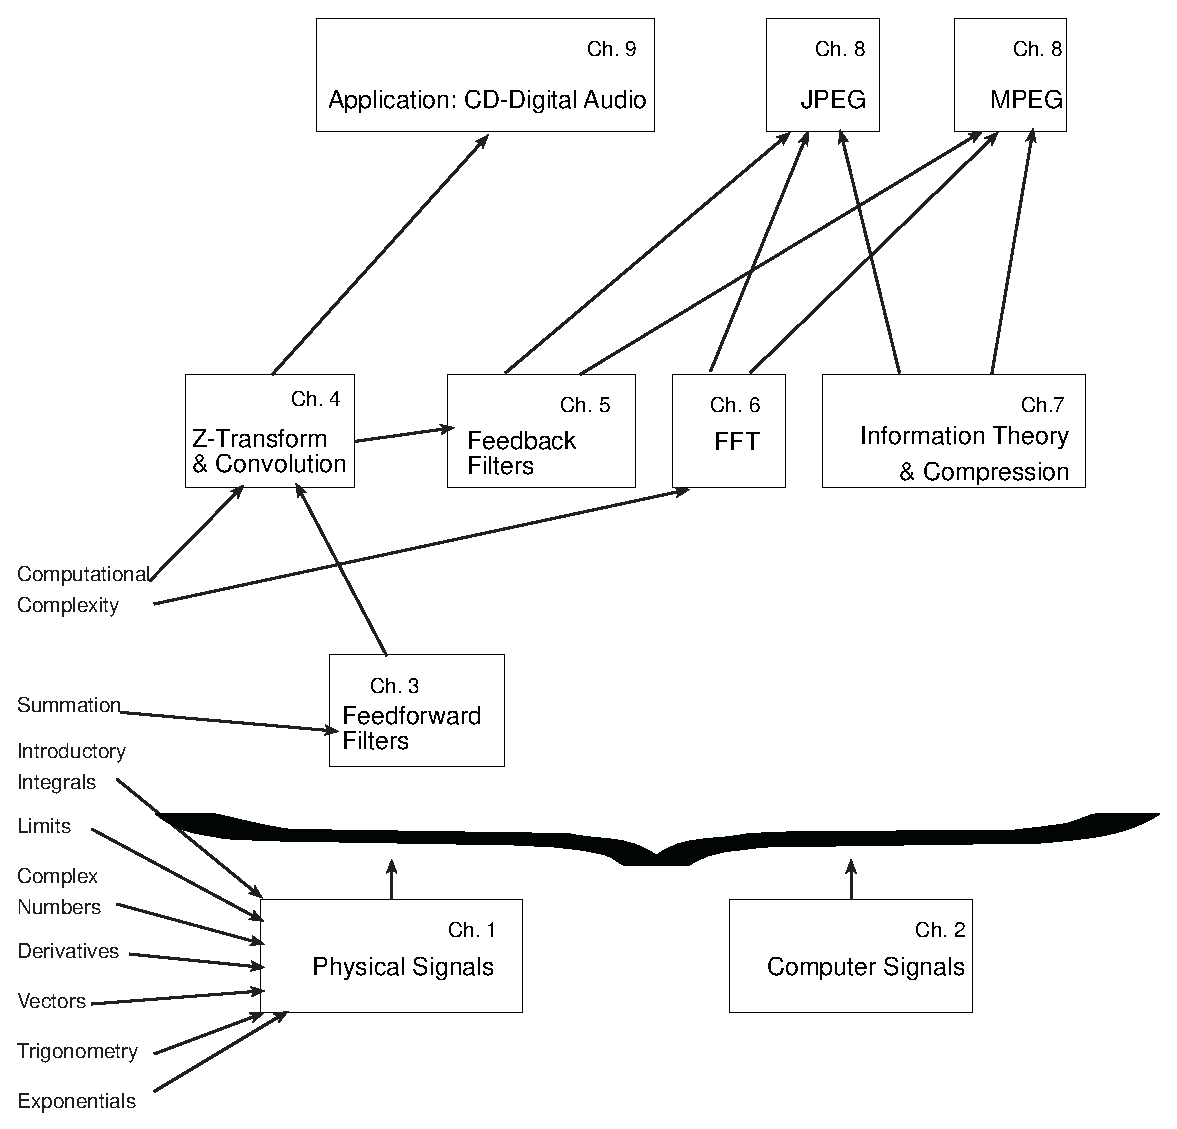
\includegraphics[width=0.9\textwidth]{roadmap}}
\caption[Course conceptual road map]{Course conceptual road
map and background knowledge.\label{fg:roadmap}}
\end{figure}

Figure~\ref{fg:roadmap} also outlines how each chapter's concepts are
used by subsequent ones and what the major themes are. You'll notice
that there's not much in the way of programming indicated. While there
\emph{is} an expectation that you understand the basics of
computational complexity and can understand, appreciate, and analyze
algorithms, this is \emph{not} a programming book. Instead, this is a
book that makes concrete many of the previously abstract mathematical
concepts that you are familiar with. It shows how these concepts
relate to \emph{real} applications that produce tangible changes on
digital signals --- it connects \emph{mathematics} to \emph{bits}.

As such, this book and the concepts within can be learned without any explicit 
knowledge of low level programming in languages like C, C++, or Java. Most of the 
exercises use an online, free tool known as Java Digital Signal Processing (J-DSP)
in order to put together block diagrams using signal processing techniques.
Most of the problems involving J-DSP require no background in any type of programming.  

However, we also provide problems for students that have varying 
levels of programming expertise (for example, you may have already taken an 
algorithms or data structures class). If you have some programming expertise, 
we provide problems that use simple Java methods (or functions) in the J-DSP environment. 
J-DSP provides a coding template for you to use, in which you can fill in
your own simple manipulations of variables in the J-DSP environment
using JAVA and use block diagrams to manipulate signals further. 
In this way, you can focus on the implementation of different algorithms, 
not the overhead involved in getting code to work.
If you have more experience in programming, we provide 
problems asking you to write
small programs in your choice of a ``lower level'' language (such as
C, C++, or Java). 

\section*{About This Book}

This book is divided into nine chapters. Chapters include self-test
exercises scattered throughout, so I suggest that you go through all
the material sequentially (or, at least, do the self-test exercises in
each section).  Each chapter concludes with written or programming
assignments and pointers to additional readings.

\index{PDF}
If you read the PDF version of this book in Acrobat
Reader, you will find that it is extensively hyper-linked.  This
includes links from exercises to their answers, links to
resources on the course web site, and links from the table of
contents, list of figures, index, etc. to their respective locations.

Note that this book is still in testing; consider it a late beta
version. Please let me know if you find any errors, omissions, or lack
of clarity.

\subsection*{Typographical Conventions}

There are no real ``standards'' for much of the notation that is used
in digital signal processing; depending on which textbook you read,
you will encounter different typographical conventions. In this
textbook, I have chosen the following:
\begin{center}
\begin{tabular}{lp{5in}}
  $j$    & $\sqrt{-1}$ \\
  $t$    & continuous time; units typically seconds \\
  $x(t)$ & a real-valued function of continuous time (physical signal) \\
  $f$    & continuous frequency; units cycles/second or Hertz (Hz) \\
  $T$    & an interval of time; often $T=1/f$, meaning the period of a
           signal \\
  $f_0$  & a particular frequency; subscript may vary depending on use \\
  $\omega$ & continuous angular frequency; units radians/second \\
  $\omega_0$ & a particular angular frequency; subscript may vary
               depending on use \\
  $n$    & discrete time or sample number; dimensionless, but you can
           think of the units as being ``samples'' \\
  $x[n]$ & a function of discrete time; may be real-valued (sampled
           signal) or discrete valued (quantized/digital signal) \\
  $\hat{f}$ & discrete frequency; units cycles/sample \\
  $\hat{f}_0$  & a particular discrete frequency; subscript may vary
                 depending on use \\
  $\hat{\omega}$ & discrete angular frequency; units radians/sample \\
  $\hat{\omega}_0$ & a particular discrete angular frequency; subscript may vary
               depending on use \\
\end{tabular}
\end{center}

\section*{Further Reading}

An excellent introduction to digital signal processing that is
targeted at beginning electrical engineering students is , \textit{DSP
  First: A Multimedia Approach}, by James H McClellan, Ronald
W. Schafer, and Mark A. Yoder (Prentice Hall, 1998).  It is important
to note that that book's target is the design of low-level signal
processing components (i.e., filters) and more generally linear,
time-invariant systems, rather than the role such components play in
overall software systems.
